% Flo
\section{Introduction to Transaction Processing}
We consider here a \textbf{multiuser} DBMS. We then have concurrent accesses to the database. The model we treat in this chapter is \textbf{interleaved concurrency}~: the concurrent execution of processes is interleaved. It allows us to keep the CPU busy when a process requires an I/O operation. \\

A \textbf{transaction} is an executing program that forms a logical unit of database processing. It includes one or more database access operations. The transaction boundaries can be \textit{explicit} by specifying \textbf{begin transaction} and \textbf{end transaction} statements or \textit{implicit} because it is embedded within an application program. \\

The database model we consider is simplified. The DB is represented as a collection of \textit{named data items}. The size of a data item is called its \textbf{granularity}. A DB item can be an \textit{attribute value}, a \textit{database record} or a \textit{disk block} (in ascending granularity). \\

Basic database access operations that may be included in a transaction~:

\begin{itemize}
    \item \textbf{read\_item(X)}. Reads a DB item named X into a program variable, let us assume it is also named X.
    \item \textbf{write\_item(X)}. Writes the value of program variable X into the database item named X.
\end{itemize}

The \textbf{read-set} of a transaction T is the set of all items that T reads, and the \textbf{write-set} is the set of all items that T writes.

\subsection{Why Concurrency Control is Needed}
Different problems may occur if no concurrency control is used.

\begin{itemize}
    \item \textbf{The Lost Update Problem}. It occurs when two transactions accessing the same DB items have their operations interleaved such that the value of some DB items becomes incorrect. For instance $T_1$ changes the value of X and $T_2$ (that must occur after $T_1$) reads this value. If an interleaving yields a read of X by $T_2$ before $T_1$ has changed X, $T_2$ reads an incorrect value.

    \item \textbf{The Dirty Read Problem}. It occurs when $T_1$ updates X and then $T_1$ fails. Meanwhile, X is accessed by $T_2$ \textbf{before} X is rolled back because of the failure. $T_2$ then reads a \textit{dirty data}.

    \item \textbf{The incorrect Summary Problem}. It occurs when $T_1$ is calculating an aggregate summary function on a number of DB items while $T_2$ is updating some of these items. Wrong values are then aggregated by $T_1$.

    \item \textbf{The Unrepeatable Read Problem}. It occurs when $T_1$ reads two times a DB item X and $T_2$ updates the value of X between the two reads.
\end{itemize}

\subsection{Why Recovery is Needed}
When a transaction $T$ is finished~:
\begin{itemize}
    \item if all the operations in $T$ are completed successfully, their effect is recorded permanently in the DB. This is a \textbf{commit}.
    \item Otherwise the operations in $T$ do not have any effect on the DB. This is an \textbf{abort}.
\end{itemize}

There are different types of failure that a DB can encounter.

\begin{itemize}
    \item Computer system crash
    \item Transaction error either because of system error or DB error (e.g. division by 0 or data not found).
    \item Concurrency control enforcement
    \item Physical problem such as disk failure, fire, explosion, Armageddon.
\end{itemize}

\section{Transaction and System Concepts}
A transaction $T$ can be in different states, as presented in figure~\ref{fig:chap20-transaction-states}. First $T$ is active to perform DB operations. When $T$ ends it is \textit{partially committed} and then is finally committed. If a problem occurs at any time before this point, $T$ fails. Eventually $T$ is terminated. In case of failure, $T$ must be \textbf{rolled back}, i.e. any changed that $T$ may have applied to the DB must be undone.

\begin{figure}[h!]
    \centering
    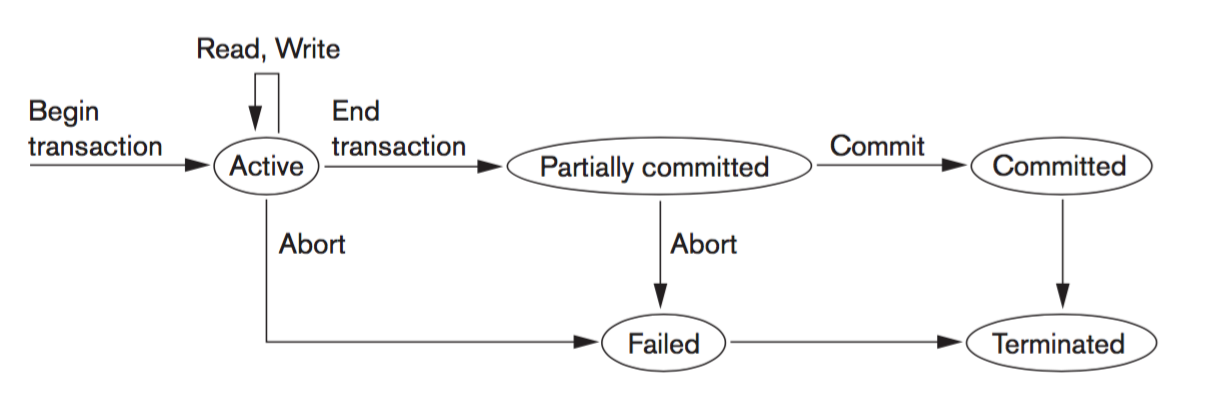
\includegraphics[scale=0.3]{chap20-transaction-states.png}
    \caption{State diagram illustrating the states for transaction execution}
    \label{fig:chap20-transaction-states}
\end{figure}

\subsection{The System Log}
The log is a sequential, append-only file kept on disk to keep track of all transaction operations. There are five possible actions to be recorded on the log.

\begin{itemize}
    \item \textbf{[start\_transaction, $T$]}. $T$ has started execution
    \item \textbf{[write\_item, $T$, $X$, old\_value, new\_value]}. $T$ has changed the value of $X$ from old\_value to new\_value.
    \item \textbf{[read\_item, $T$, $X$]}. $T$ has read the value of $X$.
    \item \textbf{[commit, $T$]}. $T$ has completed successfully and affirms that its effect can be committed to the DB.
    \item \textbf{[abort, $T$]}. $T$ has been aborted.
\end{itemize}

A transaction $T$ reaches its \textbf{commit point} when all its operations have been executed successfully and the effect of these operations have been recorded in the log.

\subsection{DBMS-Specific Buffer Replacement Policies}

A page replacement policy is needed when all the buffers in the DBMS cache are occupied and new disk pages are required to be loaded into main memory. Here are three of them.

\begin{itemize}
    \item \textbf{Domain Separation Method}. Each domain handles one type of disk page. Uses LRU, and so is static. Dynamic variant that adds load-balancing is Group LRU.
    \item \textbf{Hot Set Method}. Used for queries that have to scan a set of pages repeatedly, e.g. JOIN. This method determines which set of disk page is needed repeatedly.
    \item \textbf{The DBMIN Method}. Uses the Query Locality Set Model which determines the pattern of page references for each algorithm for a particular type of DB operation. Allocates right number of buffers using a locality set for each file.
\end{itemize}

\section{Desirable Properties of Transactions}
Transactions should possess the ACID properties~:

\begin{itemize}
    \item \textbf{Atomicity}. A transaction is atomic. Enforced by the \textit{transaction recovery subsystem}.
    \item \textbf{Consistency preservation}. It should takes the DB from one consistent state to another. The programmer is responsible for this.
    \item \textbf{Isolation}. Its execution should not interfer with other transactions executing concurrently. Enforced by the \textit{concurrency control subsystem}.
    \item \textbf{Durability}. Its changes to the DB must persist and must not be lost because of any failure. Enforced by the \textit{recovery subsystem} of the DBMS.
\end{itemize}

\subsection{Levels of Isolation}
There are several levels of isolation of a transaction.

\begin{itemize}
    \item \textbf{Level 0} if it does not overwrite dirty reads of higher-level transactions.
    \item \textbf{Level 1} has no lost updates.
    \item \textbf{Level 2} has no lost updates nor dirty reads.
    \item \textbf{Level 3} as level 2, with repeatable reads in addition.
\end{itemize}


\section{Characterizing Schedules Based on Recoverability}
A \textbf{schedule} $S$ of $n$ transactions is an ordering of the operations of the transactions. We denote $r_i(X)$ and $w_i(X)$ a read and a write operation of transaction $i$ on data item $X$ respectively. \\

Two operations in a schedule are said to \textbf{conflict} if they satisfy all three of the following conditions~:
\begin{itemize}
    \item[1.] They belong to different transactions.
    \item[2.] They access the same data item $X$.
    \item[3.] At least one of the operations is $w(X)$.
\end{itemize}

A schedule $S$ is said to be a \textbf{complete schedule} if all three of the following conditions hold~:
\begin{itemize}
    \item[1.] The operations in $S$ are exactly those operations in $T_1$,...$T_n$, including a commit or abort operation as the last operation for each $T_i$ in $S$.
    \item[2.] For any pair of operations from the same $T_i$, their relative order of appearance in $S$ is the same as their order of appearance in $T_i$.
    \item[3.] For any two conflicting operations, one of the two must occur before the other in the schedule.
\end{itemize}
Conditions 2 and 3 enforce a \textbf{total order} for any pair of conflicting operations and for any pair of operations from the same $T_i$ respectively. Nothing is required on non-conflicting operations not in the same transaction and so they follow a \textbf{partial order}.

\subsection{Characterizing Schedules Based on Recoverability}
A schedule $S$ is \textbf{recoverable} if no transaction $T$ in $S$ commits until all transactions $T'$ that have written some item $X$ that $T$ reads have committed. We said that $T$ reads from $T'$ if $X$ is first written by $T'$ and later read by $T$. \\

A schedule $S$ is \textbf{cascadeless} if every $T$ in $S$ reads only items that were written by committed transactions. \\

A schedule $S$ is \textbf{strict} if every $T$ can can neither read nor write an item $X$ until the last transaction that wrote $X$ has committed or aborted. \\

Suppose we have $n$ transactions $T_1, \dots ,T_n$. The set of \textit{all possible schedules} can be divided into two disjoint subsets~: recoverable and nonrecoverable. Also we have strict schedules $\subseteq$ cascadeless schedules $\subseteq$ recoverable schedules.

\begin{eqnarray*}
S_a &:& r_1(X); r_2(X); w_1(X); r_1(Y); w_2(X); c_2; w_1(Y); c_1; \\
S_b &:& r_1(X); w_1(X); r_2(X); r_1(Y); w_2(X); c_2; a_1;
\end{eqnarray*}

Let us consider the schedules $S_a$ and $S_b$ above where $c_i$ corresponds to the commit of $T_i$ and $a_i$ to the abort of $T_i$. Schedule $S_a$ is recoverable but $S_b$ is not. Indeed $T_2$ reads $X$ from $T_1$ but $T_2$ commits before $T_1$.

\section{Characterizing Schedules Based on Serializability}
A schedule $S$ is \textbf{serial} if for every $T \in S$ all the operations of $T$ are executed consecutively in $S$. We can make the assumption that every serial schedule is correct. The problem with these schedules is that it prevents any interleaving of operations. For instance if $T$ waits for an I/O operation we cannot switch the CPU to another $T'$. \\

A schedule $S$ is \textbf{serializable} if it is equivalent to some serial schedule. But how to define equivalence between schedules ? \\

Two schedules $S_1$ and $S_2$ are \textbf{result equivalent} if they produce the same final state of the database. The problem with this definition is that $S_1$ and $S_2$ may accidentally produce the same final DB state, as illustrated in figure~\ref{fig:chap20-result-equivalence}. Indeed if $X$ is 100 at the beginning, the two final DB states are identical. \\

\begin{figure}
    \centering
    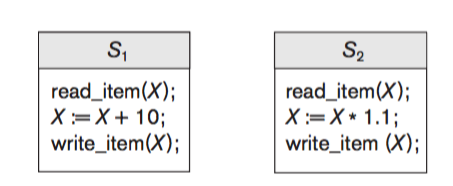
\includegraphics[scale=0.4]{chap20-result-equivalence.png}
    \caption{Result equivalence issue}
    \label{fig:chap20-result-equivalence}
\end{figure}

\textbf{Conflict Equivalence}. Two schedules are \textbf{conflict equivalent} if the relative order of any two conflicting operations is the same in both schedules. A direct consequence is that two conflict equivalent schedules yield the same final DB state. This definition is the more commonly used one. \\

\textbf{Conflict serializable Schedules}. A schedule $S$ is \textbf{conflict serializable} if it is conflict equivalent to some \textit{serial} schedule $S'$.


\subsection{Testing for Conflict Serializability of a Schedule}
There is a simple algorithm for determining wether a particular schedule is conflict serializable or not. However most concurrency control methods do \textbf{not} test for conflict serializability. But this algorithm helps to understand the chapter on concurrency control protocols.\\

The algorithm constructs a \textbf{precedence graph} which is a directed graph $G=(N,E)$ where $N = \{T_1,\dots,T_n\}$ is the set of nodes and $E=\{e_1,\dots,e_m\}$ is the set of directed edges. \\

\textbf{Algorithm}
\begin{itemize}
    \item[1.] $\forall~T_i \in S$ create a node labeled $T_i$ in the precedence graph.
    \item[2.] For each case in $S$ where $T_j$ executes a DB operation after $T_i$ executes another DB operation where at least one of the two operations is a \texttt{write(X)}, create an edge ($T_i \rightarrow T_j$).
    \item[3.] $S$ is conflict serializable if and only if the precedence graph has no cycles.
\end{itemize}

Note that there is a directed edge ($T_i \rightarrow T_j$) if and only if a pair of conflicting operations exist in $T_i$ and $T_j$ and the one in $T_i$ appears in $S$ \textit{before} the one in $T_j$. Also, this edge means that $T_i$ must come before $T_j$ in any serial schedule equivalent to $S$. So if there is no cycle in the graph, we can create an equivalent serial schedule $S'$ by ordering the transactions in $S$ as described above.

\subsection{How Serializability is Used for Concurrency Control}
A \textit{serializable} schedule has an advantage over a \textit{serial} schedule~: it uses interleaving to use the CPU as much as possible. But testing for serializability is difficult and so DBMSs use \textbf{protocols} that ensures serializability of all schedules in which the transactions participate. Chapter~\ref{chap-concurrency-control} presents concurrency control protocols that guarantee serializability.


\subsection{View Equivalence and View Serializability}
Two schedules $S$ and $S'$ are \textbf{view equivalent} if the following three conditions hold~:

\begin{itemize}
    \item[1.] The same set of transactions participates in $S$ and $S'$.
    \item[2.] For any $r_i(X)$ in $S$, if the value of $X$ has been written by $w_j(X)$, the same condition must hold for the value of $X$ read by $r_i(X)$ in $S'$.
    \item[3.] If $w_k(Y)$ is the last \texttt{write} of $Y$ in $S$, then $w_k(Y)$ must also be the last \texttt{write} of $Y$ in $S'$.
\end{itemize}

The idea is that as long as each \texttt{read} operation reads the result of the same \texttt{write} operation in both schedules, the \texttt{write} operations of each transaction must produce the same results. \\

A schedule $S$ is \textbf{view serializable} if it is view equivalent to a \textit{serial} schedule. \\

Any conflict-serializable schedule is also view serializable. However, if there is no \textbf{blind write} both definitions become equivalent. A \textbf{blind write} is a write operation in a transaction $T$ on an item $X$ that is not dependent on the old value of $X$, i.e. it is not preceded by a read of $X$ in $T$. For instance schedule $S_g$ defined below, $w_2(X)$ and $w_3(X)$ are blind writes.

$$S_g: r_1(X); w2_(X); w_1(X); w_3(X); c1; c2; c3;$$


\section{Transaction Support in SQL}
There is no explicit \texttt{Begin\_Transaction} in SQL to initiate a transaction. It is done implicitly when particular SQL statements are encountered. However, either a COMMIT or a ROLLBACK statement must end the transaction. Every transaction has 3 characteristics that may be specified~:

\begin{itemize}
    \item \textbf{Access mode} is READ ONLY or READ WRITE. Default mode is READ WRITE unless an isolation level of READ UNCOMMITTED is specified, then READ ONLY is assumed.
    \item \textbf{Diagnostic area size} is an integer $n$ that indicates the number of conditions held simultaneously in the diagnostic area. These supply feedback information for the user on the $n$ most recently executed SQL statements.
    \item \textbf{Isolation level} is READ UNCOMMITTED, READ COMMITTED, REPEATABLE READ or SERIALIZABLE. Default level is SERIALIZABLE. This is the highest level.
\end{itemize}

\begin{samepage}

If an isolation level different from SERIALIZABLE is specified, one or more of the following three violations may occur~:

\begin{itemize}
    \item[1.] \textbf{Dirty read}. $T_1$ reads the update of uncommitted transaction $T_2$, then $T_2$ aborts and so $T_1$ have read an incorrect value.
    \item[2.] \textbf{Nonrepeatable read}. $T_1$ reads a value from a table. $T_2$ then updates that value and $T_1$ reads that value again and so will see a different value.
    \item[3.] \textbf{Phantoms}. $T_1$ reads a set of rows from a table, say from a SQL WHERE-clause. Suppose $T_2$ inserts a new row $r$ in that table that also satisfies the WHERE-clause used in $T_1$. The record $r$ is called the \textbf{phantom record} because it was not there when $T_1$ starts but it is there when $T_1$ ends. $T_1$ may or may not see $r$.
\end{itemize}
\end{samepage}

Table~\ref{tab:chap20-isolation} summarizes the possible violations for the different isolation levels. A Yes means that the violation is possible. \\

\begin{table}[h!]
    \centering
    \bgroup
    \def\arraystretch{1.1}
    \begin{tabular}{llll}
         & & \textbf{Type of Violation} & \\\cline{2-4}
        \textbf{Isolation level} & \textbf{Dirty read} & \textbf{Nonrepeatable read} & \textbf{Phantom} \\
        READ UNCOMMITTED & Yes & Yes & Yes \\
        READ COMMITTED & No & Yes & Yes \\
        REPEATABLE READ & No & No & Yes \\
        SERIALIZABLE & No & No & No
    \end{tabular}
    \caption{Possible violations based on isolation levels}
    \label{tab:chap20-isolation}
    \egroup
\end{table}

\textbf{Snapshot Isolation}. This is another isolation level where a transaction $T$ sees the data items it reads based on the committed values of the items in the database state when $T$ starts. This ensures that the phantom record problem does not occur since $T$ will only see the records that were committed in the DB at the time it starts. A concurrency protocol based on this concept is presented in chapter~\ref{chap-concurrency-control}.
